\documentclass{article}
\usepackage{multicol}
\usepackage{graphicx}% Include figure files
\usepackage{dcolumn}% Align table columns on decimal point
\usepackage{bm}% bold math
\usepackage{hyperref}% add hypertext capabilities
\usepackage{booktabs}
\usepackage{listings}
\usepackage{mathtools}
\usepackage{amsmath}
\renewcommand{\abstractname}{\vspace{-\baselineskip}}
\bibliographystyle{plain}
\usepackage[utf8]{inputenc}
\usepackage{verbatim} %for å inkludere filer med tegn LaTeX ikke liker
\usepackage{mathpazo}
\usepackage{float}
\usepackage{algpseudocode}
\newcommand\numberthis{\addtocounter{equation}{1}\tag{\theequation}}
\usepackage[left=20mm,right=20mm,top=33.95mm,bottom=33.95mm]{geometry} 
% Justerer bredden på columns.
\setlength{\columnsep}{1cm}

\begin{document}

\title{The ising model}
\author{Sebastian Amundsen, Marcus Berget and Andreas Wetzel}

\maketitle

\begin{abstract}

\end{abstract}

\begin{multicols}{2}

\section{Introduction}



\section{Method}

\subsection*{The analytical expressions}

We have the normalization constant Z which defines the partition function:

\begin{equation}
Z(\beta) = \sum_{s} e^{(-\beta E_s)}
\label{eq:Z}
\end{equation}

With $\beta=1/k_BT$, where T is temperature and $k_B$ is Boltzmann's constant. We can use this partition function to find the probability $P_s$ of finding a system in a state s:

\begin{equation}
P_s=\frac{e^{-(\beta E_s)}}{Z}
\label{eq:P_s}
\end{equation}

Where $E_s$ is the energy in a given state. We have that the mean energy $E_m$ is given by:

\begin{equation}
E_m = \sum_s \frac{E_s e^{-(\beta*E_s)}}{Z}
\label{eq:E_m}
\end{equation}

The mean energy can be used to find the energy variance $\sigma_E^2$:

\begin{equation}
\begin{split}
\sigma_E^2 &= \langle E^2 \rangle - \langle E \rangle^2 \\
&= \sum_s \frac{E_s^2 e^{-(\beta*E_s)}}{Z} - \bigg(\sum_s \frac{E_s e^{-(\beta*E_s)}}{Z}\bigg)^2
\end{split}
\label{eq:E_v}
\end{equation}

This variance can give us the heat capacity $C_v$ of the system:

\begin{equation}
C_v = \frac{1}{kT} \sigma_E^2 
\label{eq:C_v}
\end{equation}

We have that the mean magnetization $\langle M \rangle$ is given by:

\begin{equation}
\langle M \rangle=\sum_s^M M_s P_s(\beta)=\frac{1}{Z}\sum_s^M M_s e^{-(\beta E_s)}
\label{eq:mM}
\end{equation}

Where $M_s$ is the different magnetizations. We have that the corresponding magnetic variance is given by:

\begin{equation}
\begin{split}
\sigma_M^2&=\langle M^2 \rangle-\langle M \rangle^2 \\
& = \frac{1}{Z}\sum_s^M M_s^2 e^{-(\beta E_s)}
\end{split}
\label{eq:M_v}
\end{equation}

We can use the magnetic variance to find the susceptibility $\chi$:

\begin{equation}
\chi = \frac{1}{k_BT}\sigma_M^2
\label{eq:chi}
\end{equation}

\subsection*{Specific case for a 2 X 2 lattice}

We can use our analytical expressions in conjunction with some periodic boundary conditions. We assume two spins in each dimension L=2. If we draw up each lattice with the different spin orientations we can find the degeneracy, energy and magnetization for each state. These values can be used to find the analytical expressions with periodic boundary conditions. We have five different spin orientations if we are studying the spin structures in Figure \ref{fig:spinn}. The energy differences $\Delta E$ in such a structure is given by:

\begin{equation}
\Delta E = E_2 - E_1 =  2J s_l^1\sum_{<k>}^N s_k
\label{eq:dE}
\end{equation}

where $E_2$ is the energy after, $E_1$ the energy before and the sum runs  over the nearest neighbors k of spin l. We can also find the difference in magnetization $\Delta M$ by only flipping the spin in the middle (dot in Figure \ref{fig:spinn}):

\begin{equation}
\Delta M = M_2-M_1=\pm2
\label{eq:dM}
\end{equation}

Where $M_2$ is the magnetization after and $M_1$ is the magnetization before we flip the spin. We can see that the change in magnetization is always $\Delta M=\pm2$, given that we only have spin configurations L=$\pm1$. These expressions are only valid as long as we have zero magnetic field. 

\subsection*{Metropolis algorithm}

We wish to find the energy differences and the change in magnetization as we run through our simulation. It is beneficial to find the energy differences before we do the metropolis sampling. Since we are only flipping one spin at a time, it is possible to find and store all the energy differences in an array as $e^{\beta\Delta E}$. This saves a lot of time, as we don't have to evaluate the exponentials in the Monte Carlo sampling. 

The metropolis algorithm only considers ratios between probabilities, which means that we do not need to calculate the partition function at all when we are using the algorithm \cite{94}. 

\section{Results}

\begin{table}[H]
\begin{center}
\caption{Energy and magnetization given number of up spins.}
\begin{tabular}{  |c|c|c|c|c|c| } \hline
$N_{\text{spins up}}$&Degeneracy&E&M \\ \hline
4&1&-8 J&4\\ \hline
3&4&0 &2 \\ \hline
2&4&0&0\\ \hline
2&2&8 J&0\\ \hline
1&4&0&-2\\ \hline
0&1&-8 J&-4\\ \hline
\end{tabular}
\label{tab:up_spins}
\end{center}
\end{table}

In Table \ref{tab:up_spins} we have the energy and magnetization given the number of up spins. 

\subsection*{Specific case for a 2 X 2 lattice}

\begin{equation}
Z=4\cosh{(8J\beta)}+12
\label{eq:Z_22}
\end{equation}

We have that the partition function for our specific $2\times2$ lattice case is given by equation \ref{eq:Z_22}.

\begin{equation}
E_m=-8\bigg(\frac{\sinh{(8J\beta)}}{\cosh{(8J\beta)}+4}\bigg)
\label{eq:E_22}
\end{equation}

The mean energy is given by equation \ref{eq:E_22}.

\begin{equation}
\begin{split}
C_v = \frac{1}{kT} \bigg({4cosh(8\beta)+12}\\
-\bigg(\frac{-8\sinh{(8J\beta)}}{\cosh{(8J\beta)}+3}\bigg)^2\bigg)
\end{split}
\label{eq:Cv_22}
\end{equation}

The heat capacity is given by equation \ref{eq:Cv_22}.

\begin{equation}
\langle M \rangle=0
\label{eq:M_22}
\end{equation}

The mean magnetization is given by equation \ref{eq:M_22}.

\begin{equation}
\chi = \frac{1}{kT} \bigg(\frac{32e^{8\beta}+128}{4cosh+12}\bigg)
\label{eq:chi_22}
\end{equation}

The susceptibility is given by equation \ref{eq:chi_22}. All the calculations are given in appendix B.

In the $2\times2$ lattice case there are only five possible values for the energy difference. These are given in section \ref{eq:calc_dE} in appendix B.

\section{Discussion}

\section{Concluding remarks}

\end{multicols}

\clearpage

\appendix % Her kommer appendix.

\section{Appendix}

\begin{figure}[H]
	\centering
	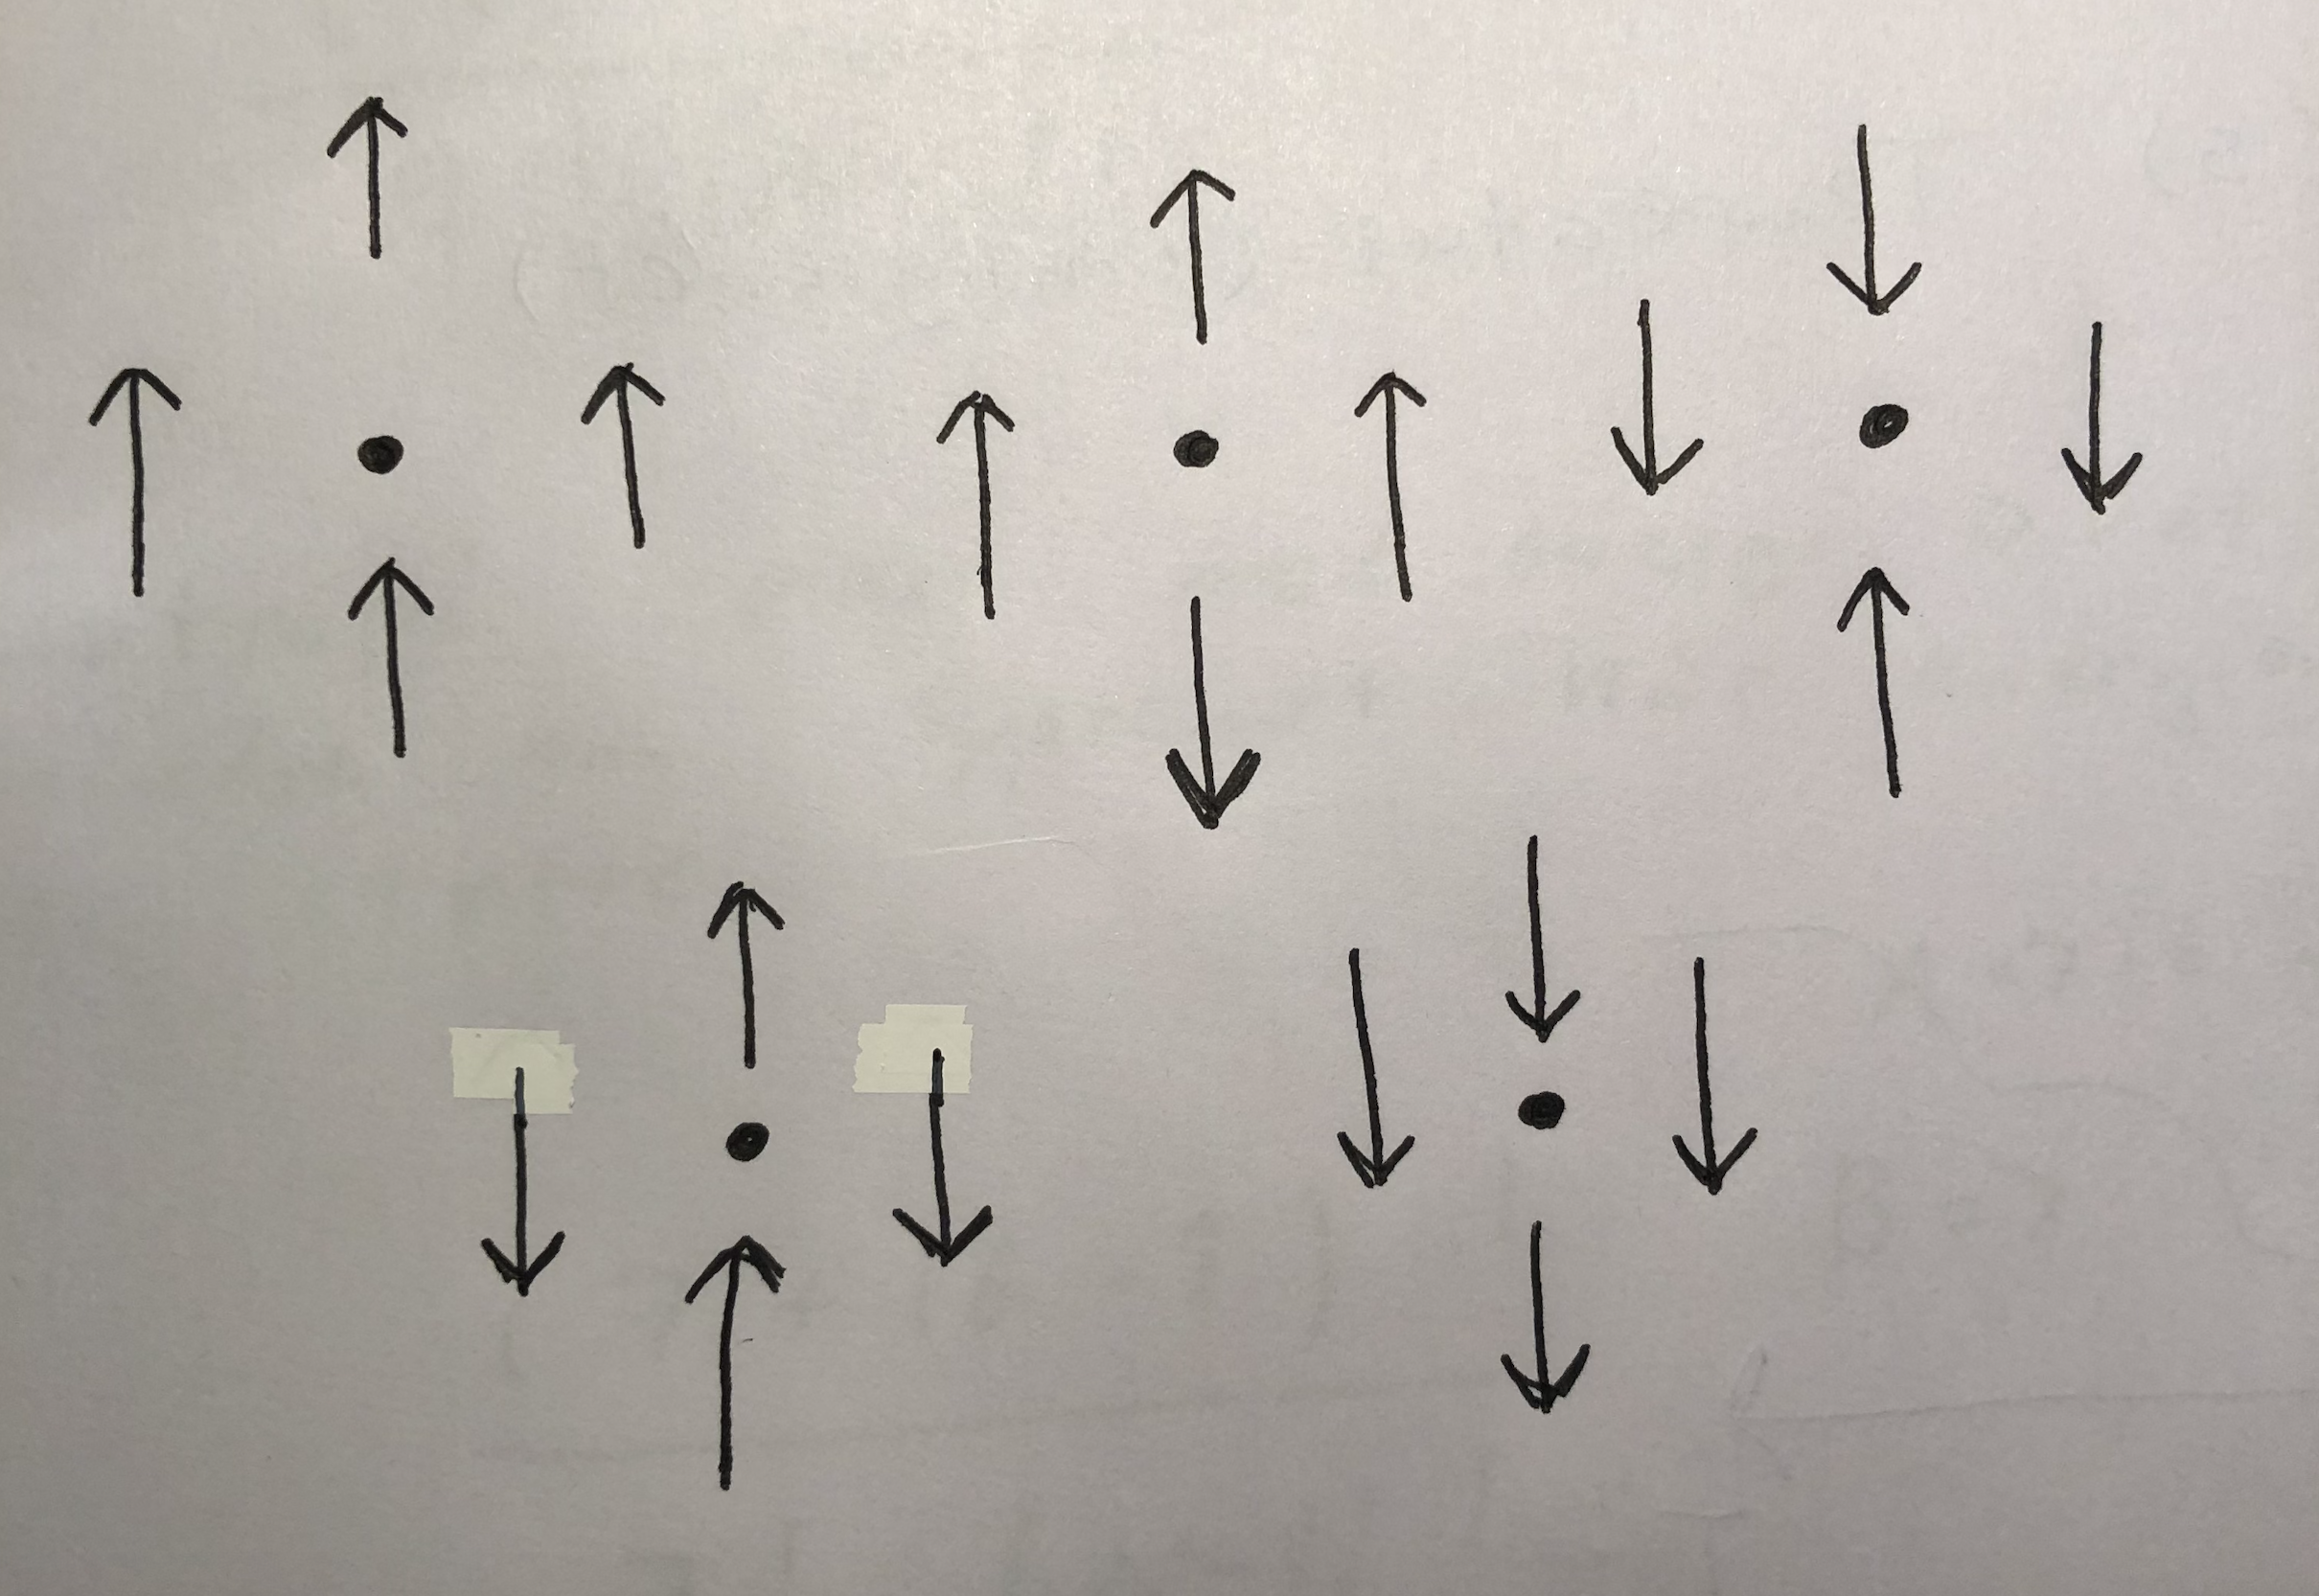
\includegraphics[width=100mm]{Spin}
	\caption{The different spin orientations.}
	\label{fig:spinn}
\end{figure}

\section{Appendix}
\subsection*{Analytical expression}

The partition function for the $2\times2$ lattice is given by equation \ref{eq:Z}:

\begin{equation}
\begin{split}
Z&=2e^{8J\beta}+2e^{-8J\beta}+12e^0\\
&=4\cosh{(8J\beta)}+12
\end{split}
\label{eq:calc_Z}
\end{equation}

This expression combined with equation \ref{eq:E_m} gives the energy:

\begin{equation}
\begin{split}
E_m &= \frac{2\times8Je^{-8J\beta}-2\times8Je^{8J\beta}}{Z}\\
&=\frac{-16J(e^{8J\beta}-e^{-8J\beta})}{Z}\\
&=\frac{-32\sinh{(8J\beta)}}{4\cosh{(8J\beta)}+12}\\
&=-8\bigg(\frac{\sinh{(8J\beta)}}{\cosh{(8J\beta)}+3}\bigg)
\label{eq:calc_E}
\end{split}
\end{equation}

We also have a variance $<\sigma_E^2>$ which we find by using equation \ref{eq:E_v}:

\begin{equation}
\begin{split}
<\sigma_E^2>&=\bigg(\frac{2\times(-8)^2e^{-(-8\beta)} + 2 \times (8)^2e^{-(8\beta)}}{Z}\bigg)-E_m^2\\
&=\frac{128(e^{8\beta}+e^{-8\beta})}{Z}-E_m^2=\frac{256\cosh{(8\beta)}}{4cosh(8\beta)+12}-\bigg(\frac{-8\sinh{(8J\beta)}}{\cosh{(8J\beta)}+3}\bigg)^2
\label{eq:calc_Ev}
\end{split}
\end{equation}

Which gives us the heat capacity $C_v$ by using equation \ref{eq:C_v}:

\begin{equation}
C_v = \frac{1}{kT} \bigg({4cosh(8\beta)+12}-\bigg(\frac{-8\sinh{(8J\beta)}}{\cosh{(8J\beta)}+3}\bigg)^2\bigg)
\label{eq:calc_Cv}
\end{equation}

We find the mean magnetization by using equation \ref{eq:mM}:

\begin{equation} \label{eq:calc_M}
\begin{split}
\langle M \rangle& = 1\times 4 \times P(-8) + 4 \times 2 \times P(0) + 4 \times 0 \\
& + 2\times0+4 \times (-2) \times P(0) +  1\times(-4) \times P(-8)\\
&=4\bigg(\frac{e^{-8J\beta }}{4\cosh{(8J\beta)}+12}\bigg)-4\bigg(\frac{e^{-8J\beta }}{4\cosh{(8J\beta)}+12}\bigg) \\
&=0
\end{split}
\end{equation}

We also have a variance $<\sigma_M^2>$ which we find by using equation \ref{eq:M_v}:

\begin{equation}
\begin{split}
<\sigma_M^2>&=\frac{1}{Z}\bigg(4^2e^{-(-8\beta)}+8^2e^0+(-8)^2e^0+(-4)^2e^{-(-8\beta)}\bigg)\\
&=\frac{16e^{8\beta}+64+64+6e^{8\beta}}{Z}=\frac{32e^{8\beta}+128}{4cosh+12}
\end{split}
\label{eq:calc_Mv}
\end{equation}

Which gives us the susceptibility $\chi$ by using equation \ref{eq:chi}:

\begin{equation}
\chi = \frac{1}{kT} \bigg(\frac{32e^{8\beta}+128}{4cosh+12}\bigg)
\label{eq:calc_chi}
\end{equation}

\subsection*{Boundary conditions and Boltzmanns distribution}

We assume that the original position of the middle spin in Figure \ref{fig:spinn} is up (the middle spin is the dot). We find the energy differences by using equation \ref{eq:dM}:

\begin{equation}\label{eq:calc_dE}
\begin{split}
&\Delta E_1 = 4-(-4)=8\\
&\Delta E_2 = 2-(-2)=4\\
&\Delta E_3 = -2-(2)=-4\\
&\Delta E_4 = 0-0=0\\
&\Delta E_5 = -4-(4)=-8\\
\end{split}
\end{equation}

We can see that we obtain five different energy differences as we flip the spin from up to down in the middle of the structures in Figure \ref{fig:spinn}.

\bibliography{References} % Kilder.
\begin{thebibliography}{9}
\bibitem{94}
	Jensen, M.H., 2015, Computational Physics Lecture Notes Fall 2015
\end{thebibliography}

\end{document}